\documentclass[a4paper,11pt]{article}
\usepackage[utf8]{inputenc}
\usepackage[italian]{babel}
\usepackage{graphicx}
\usepackage[colorlinks=true,linkcolor=blue]{hyperref}
\graphicspath{ {../app/src/main/res/mipmap-xxxhdpi/} {./images/}}

\title{Simulatore di scherma per Android\\con riconoscimento di gestures}
\author{Francesco Bultrini, matricola 278696\\
 Claudio Pannacci, matricola 283526}
\date{Anno accademico 2016-2017}

\begin{document}

\begin{figure}[t]

  \centering
  
\includegraphics{img_fency_logo}

\end{figure}

\maketitle
\newpage

\tableofcontents

\listoffigures

\newpage

\subsection{Abstract}
L'obiettivo di questo progetto è la realizzazione di un gioco  ispirato allo sport della scherma, per cellulari dotati di sistema operativo Android che, nella sua versione finale, consisterà in una sfida locale tra due giocatori dove lo scambio di informazioni avverrà tramite Bluetooth.\\ Si valuta anche la possibilità di utilizzare la tecnologia NFC per eseguire il \hyperref[pairing]{\emph{pairing}} dei dispositivi.
\newpage

\subsection{Realizzazione}
Si è deciso di utilizzare il \hyperref[spirale]{\emph{modello a spirale}} come modello di sviluppo e ad ogni ciclo verrà realizzato un prototipo.\\ Non tutte le funzionalità saranno presenti da subito ma verranno implementate in \hyperref[release]{\emph{release}} successive.\\Per la codifica è stato adottato il metodo del \hyperref[pairp]{\emph{Pair Programming}} utilizzando \href{https://developer.android.com/studio/index.html}{Android Studio} come ambiente di sviluppo.\\Il codice sorgente è pubblicato su GitHub all'indirizzo: \begin{center}
\url{https://github.com/Disorganizzazione/Fency}\\
{\footnotesize Il codice sorgente è coperto da licenza GNU.}
\end{center}
\newpage

\part{Riconoscimento delle gestures e interfaccia grafica}
\ 
\section{Analisi dei requisiti}
\subsection{Requisiti riconoscimento gesture}
Al fine di riconoscere le \hyperref[gesture]{\emph{gestures}} si deve accedere, tramite classi di sistema, ai valori di accelerometro, giroscopio e magnetometro. Per ridurre il dominio dei movimenti da analizzare, sarà necessario definire un orientamento del telefono (in direzione orizzontale, con lo schermo rivolto verso l'alto) e assicurarsi che tale stato venga mantenuto durante lo spostamento.\\ A questo scopo la classe \textbf{SensorFusion} di Paul Lawitzki, che combina i dati del giroscopio a quelli del magnetometro riducendo il rumore, permette di avere informazioni affidabili sull'orientamento del dispositivo tramite i valori di \hyperref[pra]{\emph{pitch}}, \hyperref[pra]{\emph{roll}} e \hyperref[pra]{\emph{azimuth}}. La descrizione dell'affondo si basa sui dati forniti dall'accelerometro, accessibili mediante l'implementazione dell'interfaccia \textbf{SensorEventListener}. Utilizzando la modalità \textbf{Linear Acceleration}, si hanno i valori di accelerazione sui tre assi, senza la componente gravitazionale. Il movimento dell'affondo causa un'accelerazione positiva sull'asse Y (parallelo al lato lungo del dispositivo) seguito da una accelerazione di modulo maggiore, stesso verso e direzione opposta, dovuta all'arresto del dispositivo nel momento in cui si conclude l'affondo. Inoltre, per impedire ad altri movimenti (come lo scuotimento) di essere classificati come affondi bisogna accertarsi dell'effettivo spostamento del dispositivo. Non basta quindi impostare una soglia minima di accelerazione ma è necessario anche stimare la durata del movimento.
\subsection{Requisiti interfaccia grafica}
Al fine di interagire con l'utente tramite un'interfaccia grafica, si ricorrerà alla classe di sistema \textbf{AppCompatActivity}, la quale si lega ad un \hyperref[layout]{\emph{layout}} in formato XML e viene eseguita all'apertura dell'app.\\ Il passaggio da un' attività all'altra sarà gestita implementando l'intefaccia \textbf{OnCLickListener}, la quale permette di assegnare agli oggetti visuali una funzione di risposta personalizzata.
\newpage

\section{Descrizione del codice}
Il codice presenta tre livelli: classi e interfacce di sistema, classi astratte \textbf{\emph{Fency}} e classi concrete.
\begin{figure}[h]
\caption{Digramma di classe completo}\noindent\makebox[\textwidth]{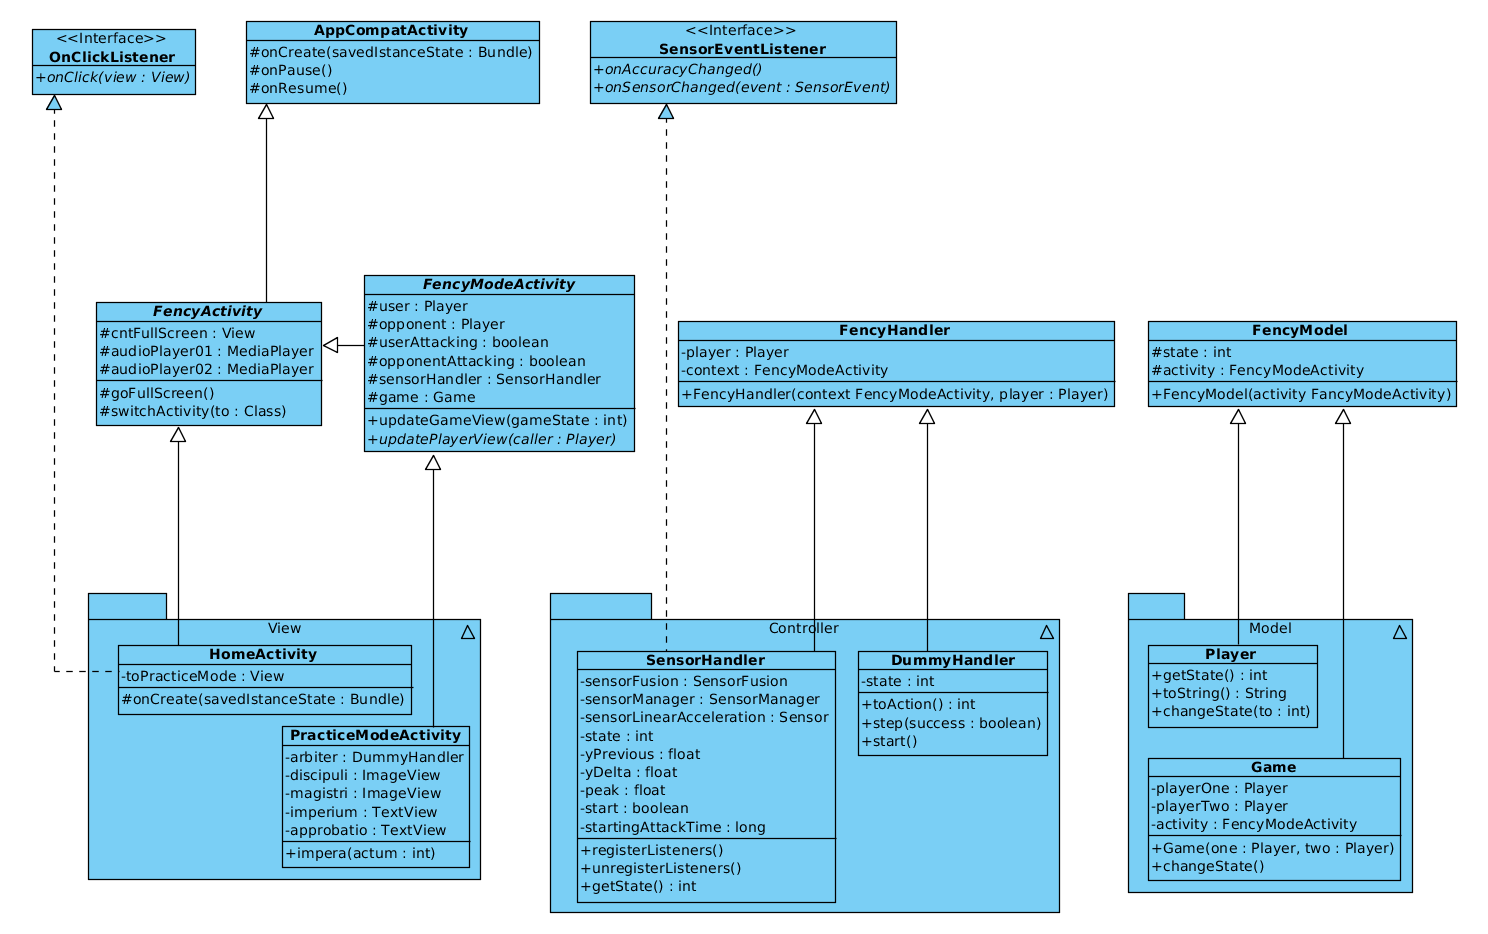
\includegraphics[width=\paperwidth]{UML_classes}}
\end{figure}
\subsection{Design pattern MVC}
Come mostrato nel diagramma, abbiamo applicato una variante del design pattern \hyperref[MVC]{\emph{Model View Controller}} nella quale il controller dei modelli giocatore (\textbf{SensorHandler}) ne modifica lo stato in base ai valori dei sensori, anzi che in risposta ad un' interazione con le loro componenti grafiche da parte dell'utente. Ogni volta che lo stato del \textbf{Player Model} cambia, esso chiama la funzione \emph{updatePlayerView()} che ne aggiorna la visualizzazione. \\Similmente il \textbf{Game Model} chima la funzione \emph{updateGameView()}.
\newpage

\subsubsection{Relazione tra i Model}
Ogni volta che un giocatore passa ad uno stato di attacco, il \textbf{Player Model} chiama la funzione \emph{ChangeState()} del \textbf{Game Model}: esso controlla gli stati di entrambi i giocatori e si aggiorna.
\begin{figure}[!h]
\caption{Diagramma di stato e di sequenza per la classe Player}
\ \\\noindent\makebox[\textwidth]{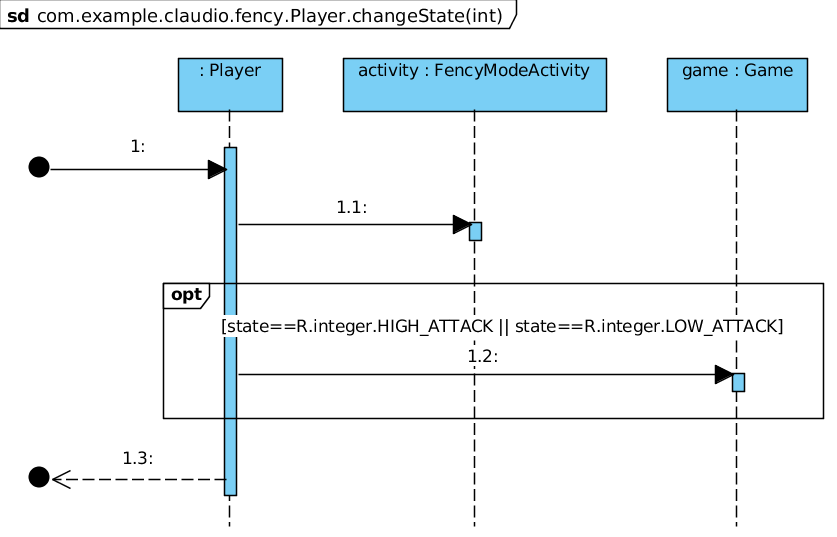
\includegraphics[scale=0.4]{PlayerChangeState} \ \ \ \ \ \ \ \ 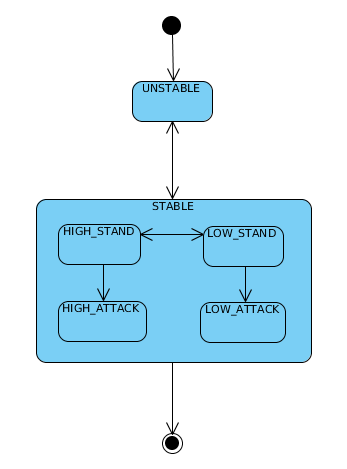
\includegraphics[scale=0.42]{PlayerStates}}
\end{figure}
\begin{figure}[!h]
\caption{Diagramma di stato e di sequenza per la classe Game\ \ \ }\ \\
\noindent\makebox[\textwidth]{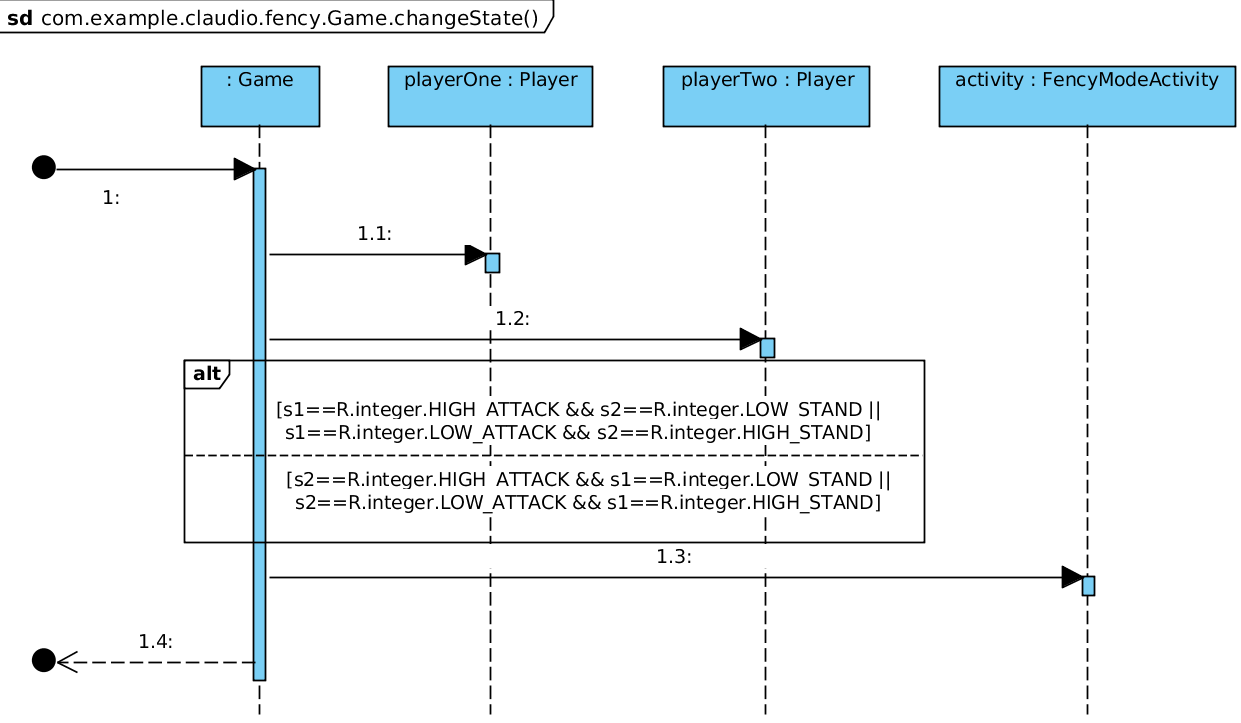
\includegraphics[scale=0.3]{GameChangeState}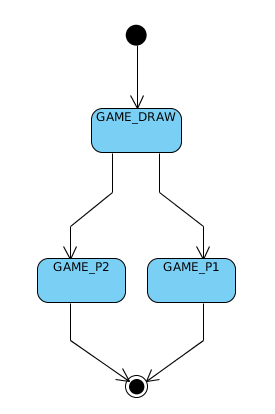
\includegraphics[scale=0.5]{GameStates}}
\end{figure}
\newpage

\subsection{La classe SensorHandler}

\begin{figure}[h]
\caption{Diagramma di attività: SensorHandler.onSensorChanged()}\noindent\makebox[\textwidth]{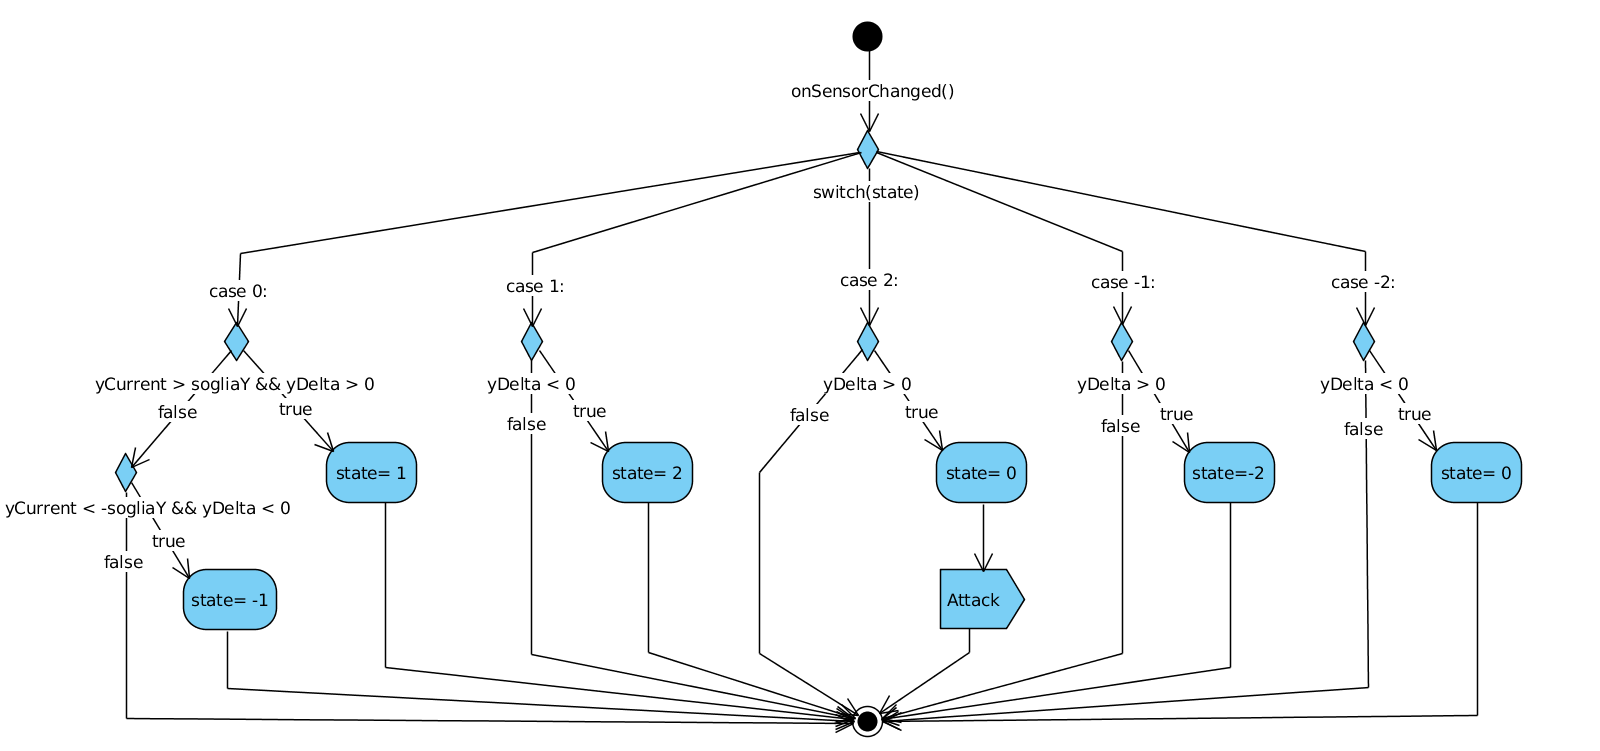
\includegraphics[width=\paperwidth]{SensorHandler}}
\end{figure}

\subsubsection{Casi di test funzionali}
\begin{tabular}{  l|*{2}{c}|r  }
N & Pitch & Roll & Validità\\
\hline
1 & -30 & 0 & Valido\\
2 & -70 & 0 & Non valido\\
3 & 5 & 0 & Non valido\\
4 & -30 & -8 & Non valido\\
5 & -30 & 8 & Non valido\\
\end{tabular}
\subsubsection{Casi estremi}
\begin{tabular}{ l| c r }
& Validi & Non valdidi\\
\hline
Pitch & -60 + DOUBLE_MIN , -5 - DOUBLE_MIN &  -60, -5\\
Roll & -5, 5 & -5 - DOUBLE_MIN, 5 + DOUBLE_MIN\\
\newpage

\section{Meccaniche di gioco}
Il gioco prevede che l'utente sia possibilmente in piedi e tenga con una mano il dispositivo davanti a sé: da questa posizione può alternarsi rapidamente fra i due stati di guardia HighStand e LowStand semplicemente regolandone il pitch.
Partendo da una di queste posizioni è possibile, mimando un affondo con la dovuta velocità, raggiungere rispettivamente gli stati HighAttack e LowAttack.
\begin{figure}[h]
\caption{Casi d'uso: posizioni del giocatore}
\noindent\makebox[\textwidth]{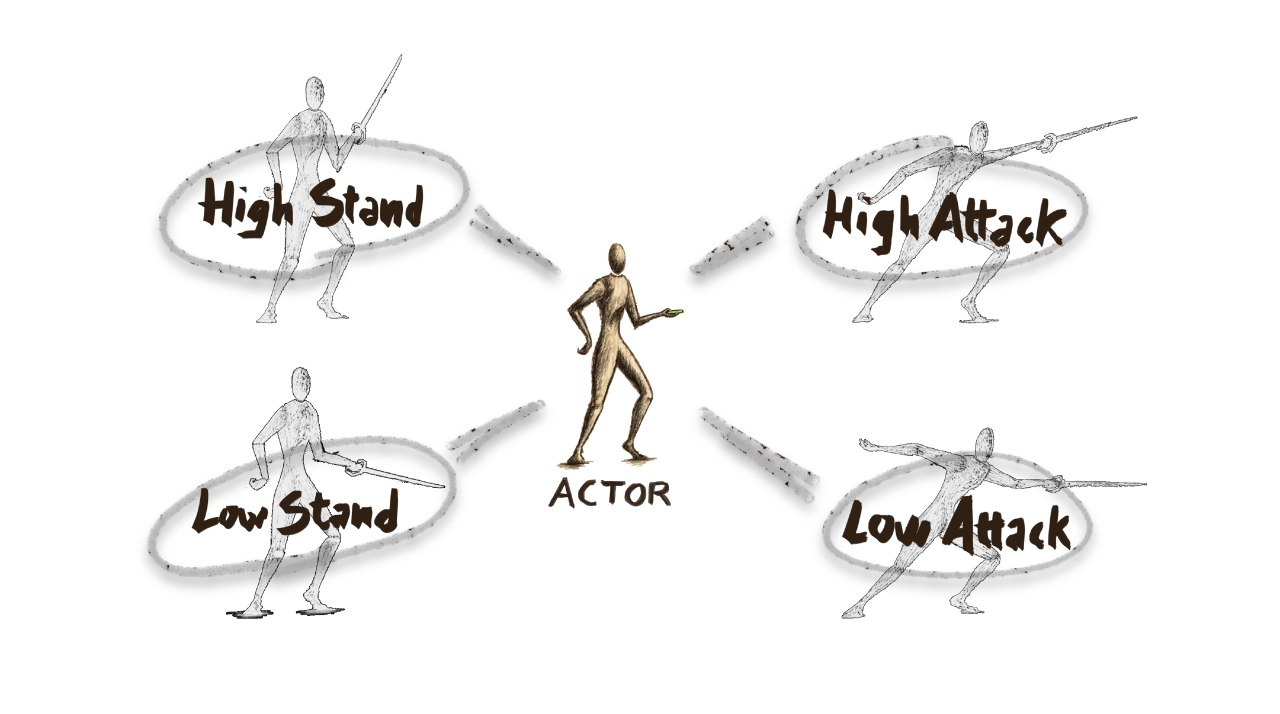
\includegraphics[scale=0.5]{UseCases}}
\end{figure}
\subsection{Scopo del gioco}
Lo scopo del gioco è colpire l'avversario attaccandolo all'altezza opposta alla sua guardia.
Al contrario, vi è parità nello scambio di colpi quando le due "spade" si scontrano virtualmente: un attacco può essere quindi deflesso sia correggendo lo stato di guardia in base all'attacco in arrivo, sia compiendo un attacco alla stessa altezza dell'avversario.
\newpage

\renewcommand\thesection{}
\section{Glossario}
\ \\
\textbf{Gesture}: specifico movimento del dispositivo\\ \label{gesture}\textbf{Layout}: disposizione grafica degli elementi\\ \label{layout}\textbf{Pairing}: connessione reciproca tra due dispositivi\\ \label{pairing}\textbf{Release}: rilascio del software\\ \label{release}\textbf{Pitch, Roll, Azimuth}: (come in figura)\\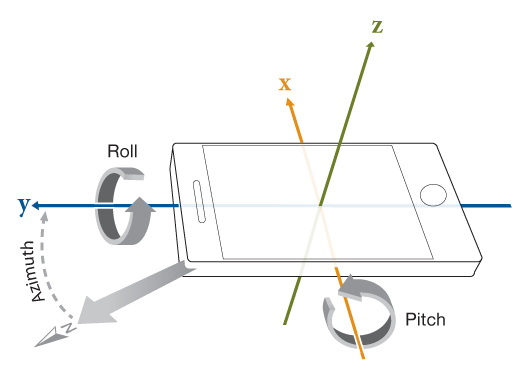
\includegraphics[scale=0.5]{PitchRollAzimuth}\\ \label{pra}\textbf{Modello a spirale}: modello di cilco di vita del software proposto da Barry Boehm nel 1988 \\ \label{spirale}\url{https://it.wikipedia.org/wiki/Modello_a_spirale}\\\textbf{Pair programming}: tecnica di sviluppo del software nella quale due programmatori lavorano insieme a una postazione di lavoro \\ \label{pairp}\url{https://it.wikipedia.org/wiki/Pair_programming}\\\textbf{Model View Controller (MVD)}: pattern architetturale molto diffuso nello sviluppo di sistemi software ad oggetti che separa la logica di visualizzazione di un oggetto da quella di gestione\\ \label{MVC}\url{https://it.wikipedia.org/wiki/Model-View-Controller}

  


\end{document}